\documentclass[oneside, openany]{tum-book}

\title{Predicting Bankruptcy with Machine Learning: An Undersampling and Feature Importance Approach using a Taiwanese Dataset}
\author{Niklas Demmrich}

\titledescription{Thesis
for the Attainment of the Degree\\
  \textbf{Bachelor of Science}\\
  at the Technical University of Munich}
\fineprint{%
  \textbf{Examiner}\\
  Prof. Dr. Helmut Farbmacher\\
  Chair of Applied Econometrics\\
  \vspace{12pt}
  \textbf{Supervised by}\\
  Gabriel Vollert\\
  \vspace{12pt}
  \textbf{Submitted by}\\
  Niklas Demmrich\\
  Matriculation Number: 03774170\\
  \vspace{12pt}
  \textbf{Submitted on}\\
  31.07.2026}


% --- packages added for the draft (amsmath/graphicx/pgfplots/caption already in class) ---
\usepackage{booktabs} % professional table rules (\toprule \midrule \bottomrule)
\usepackage{multirow} % \multirow cells in the confusion-matrix table

% search paths for figures -> \includegraphics needs only the filename
\graphicspath{{figures/results/}{figures/appendix/}{figures/methodology/}{tum-resources/images/}}

\begin{document}


% Abstract removed per supervisor (Gabriel): the summary + research question fold
% into the Introduction. Content kept in chapters/00_Abstract.tex as raw material;
% revisit when the Introduction is written.
%\chapter*{Abstract}
\noindent
Corporate bankruptcy prediction is complicated by severe class imbalance, and
much of the recent literature addresses this by synthesising minority
observations, reporting accuracies near $99\%$ on data that is partly fabricated.
This thesis takes the opposite approach: it trains exclusively on real
historical firms, restoring balance through cluster-centroid undersampling and
evaluating models by the recall-oriented $F_2$-score. On the Taiwanese
Bankruptcy Dataset ($6{,}819$ firms, $95$ features, $3.23\%$ bankrupt), three
models of increasing complexity are compared. Gradient boosting attains the best
cross-validated performance ($F_2 = 0.550$), ahead of a random forest ($0.546$)
and a logistic-regression baseline ($0.482$), and competitive with the
undersampling benchmark of Wang and Liu (2021) while introducing no synthetic
data. The central contribution is an interpretability layer that their work
lacked: comparing native, permutation, and SHAP importance across all three
models reveals a systematic divergence. Native impurity importance is distorted
by a known bias towards continuous features, permutation importance collapses
under the collinearity of the ratios, and SHAP --- the only method yielding
signed, comparable attributions for every model --- provides the most
trustworthy ranking, dominated by leverage and debt-servicing measures. The
thesis argues that this comparison, not any single importance list, is what
widens the black box.

\vspace{1em}
\noindent\textit{\textbf{Keywords: }bankruptcy prediction, class imbalance,
undersampling, feature importance, SHAP}

%\newpage

\tableofcontents
\listoftables
\listoffigures
\newpage


\chapter{Introduction}
\label{ch:introduction}

Corporate insolvencies are rising worldwide for the fifth consecutive year.
\textcite{allianztrade2025} expect a further increase of $5\%$ in 2026, taking
global business failures to a record level about a quarter above where they stood
before the pandemic and putting an estimated $2.1$ million jobs at risk. Behind
each of these failures stand creditors, employees, suppliers and banks who carry
the cost, which is why predicting bankruptcy early enough to react has been a
research question for decades. Machine learning has pushed this field to
remarkable reported numbers, with recent studies reaching accuracies of $98$--$99\%$
\parencite{pham2025, suresh2025, sinap2025}. Two things are troubling about these
results. First, they rest on synthetic oversampling, which balances the data by
fabricating bankruptcy events that never occurred. Second, they are produced by
models whose decisions remain largely unexplained, so even a correct prediction
gives an analyst little to work with.

This thesis takes the opposite route on both points. Using a widely studied
dataset of $6{,}819$ Taiwanese firms, of which only $3.2\%$ went bankrupt, it
trains exclusively on real observations. The imbalance is handled by
ClusterCentroids undersampling, which condenses the healthy majority into
representative real firms instead of inventing bankrupt ones. Three models of
increasing complexity, a logistic regression, a random forest and gradient
boosting, are compared under repeated stratified cross-validation and selected on
the $F_2$-score, because missing a bankruptcy costs far more than a false alarm.
The setup extends \textcite{wangliu2021}, who established this sampling and
evaluation framework on the same data but stopped at predictive performance.

The added layer is the actual contribution and leads to the research question of
this thesis, which financial features the fitted models rely on and how far the
answer depends on how one asks. Three importance methods, native importance,
permutation importance and SHAP, are applied to all three models. The short answer
is that no single ranking exists, as the methods diverge in ways their known
weaknesses predict, while a consistent signal remains, with every model placing a
measure of debt dependence at or near the top. Chapters~2 and~3 review the
literature and the data, Chapters~4 and~5 develop the methodology and the
importance methods and Chapters~6 to~8 report, discuss and conclude.
\chapter{Literature Review}
\label{ch:literature}

The quantitative prediction of corporate bankruptcy has moved through three
overlapping phases, from classical statistical models over the adoption of
machine learning to a growing concern with class imbalance and model
interpretability. This chapter reviews the literature most relevant to 
the present work and isolates the gap this thesis addresses.

The study of bankruptcy prediction initially involved \textcite{beaver1966},
who examined financial ratios one at a time to separate failing from healthy
firms. \textcite{altman1968} then combined five ratios into a single
discriminant function, the Z-score, and later \textcite{ohlson1980} advanced
the field by introducing logit models. These methods are extensively discussed in the
literature reviewed in this thesis and are therefore only briefly noted here.
What matters for the present work is their common limitation. Although these
models are transparent and have coefficients that can be easily understood in
economic terms, they assume a fixed functional form and are thus incapable of
dealing with potential non-linear interactions in the data. The study by
\textcite{liang2016} is representative of the shift towards machine learning and
is also the origin of this dataset. At the same time, \textcite[562]{liang2016}
forced the two classes into an even balance by simple stratified sampling, a
decision that has since been questioned and is a design choice this 
thesis also does not follow.

Since bankruptcies are rare, the treatment of class imbalance has turned into a
major methodological issue. \textcite{veganzones2018} demonstrate that standard
models tend to perform badly as soon as bankrupt firms start to become too rare
in the training data, which means that some kind of rebalancing is required.
There are two types of solutions and they differ according to the kind of data
the model ends up learning. The oversampling methods, of which SMOTE
\parencite{chawla2002} is the most commonly used, create additional synthetic
observations for the minority class until the classes are balanced. In contrast,
specific undersampling methods reduce the number of cases in the majority class, so
that each observation on which the model is trained actually corresponds to a
firm that really existed. This difference is the methodological commitment of
the thesis. The closest study in this area is \textcite{wangliu2021}, in which
they examine several undersampling methods on exactly the dataset used here,
combined with repeated stratified cross-validation and the $F_2$-score as the
primary metric. The best setup that they achieve, using edited nearest
neighbours with a Naive Bayes classifier, attains an $F_2$ score of
$0.423$ \parencite[12]{wangliu2021}. The sampling approach, the idea of
leakage-aware validation and the choice of metric form the base that this thesis
extends. Cluster-based undersampling in particular has already existing work
outside of \textcite{wangliu2021}, since \textcite[11]{ansahnarh2024} also keep the
cluster centroids of the majority class on the same data, making use of the same
Python implementation as is used here, even though it is part of a more complex
overall setup.

There is also a large amount of more recent research which finds much higher
performance by combining synthetic oversampling with flexible learning methods,
an approach that \textcite{liashenko2023} and \textcite{amirshahi2024} survey
across both balanced and imbalanced settings. \textcite[305]{pham2025}, who also
provide a general overview of sampling strategies, achieve accuracies close to
$98.6\%$ using SMOTE and an artificial neural network, while \textcite{suresh2025}
and \textcite{sinap2025} report similar results with similar approaches.
Nevertheless, high accuracy under these setups has to be read with care. 
Some studies balance the data before splitting it, so the models are partly 
evaluated on synthetic firms, but even when the test set instead keeps the 
natural $96.8/3.2$ class distribution, accuracy alone is misleading because a 
model that predicts every firm as non-bankrupt already achieves $96.8\%$ accuracy.
This thesis takes these studies as points of differentiation rather than as 
templates and accepts the lower reported numbers in exchange for training only 
on real firms.

The final aspect of the issue relates to the features, the financial ratios,
which are responsible for the predictions. Some studies address this by carrying
out a selection at an early stage, either by selecting the features before
training, for instance \textcite{veganzones2018} who eliminate highly correlated
ratios and \textcite{chaudhary2023} who applies a Pearson-correlation screen, or
by transforming the features, as \textcite{ko2024} and \textcite{sinap2025} do
by means of factor analysis and principal components. Even though these
filtering methods are simple, they evaluate the features before and
independently of the model, whereas this thesis is concerned with finding
out what the trained model in fact relies on. In this regard, post-hoc
importance methods have been used, as \textcite{ansahnarh2024} report
random-forest importances and \textcite{sinap2025} is the only one of the
studies looked at here that makes use of SHAP, even though each of them provides
only a single importance measure without checking whether other measures would
be in agreement. Together, the framework being trained entirely on real firms
through undersampling and the comparison of importance methods make up the gap that 
this thesis aims to address. The technical
background of these methods is given in
Chapters~\ref{ch:methodology} and~\ref{ch:featureimportance}.


% highlight more the contribution of the thesis
\chapter{Dataset}
\label{ch:dataset}

This analysis uses the Taiwanese Bankruptcy Dataset, a well-established benchmark
compiled from the Taiwan Economic Journal \footnote{\url{https://www.tejwin.com}} from 1999 to 2009 and made accessible
through the \textcite{uci_taiwan}. Corporate bankruptcy was defined based on the
rules of the Taiwan Stock Exchange.\footnote{\url{https://twse-regulation.twse.com.tw/EN/law/DOC01_print.aspx?FLCODE=FL007304&FLNO=50-1}} 
It contains $6{,}819$ companies, each described by $95$ financial attributes covering standard business performance metrics such as 
Return on Assets (ROA), the Debt Ratio, Cash Flow Rate or Earnings per Share (EPS). Outcome is simply measured by one binary variable 
of either 0 = healthy or 1 = bankrupt.

\begin{table}[htbp]
  \centering
  \caption{Composition of the Taiwanese Bankruptcy Dataset.}
  \label{tab:dataset}
  \begin{tabular}{lrr}
    \toprule
    \textbf{Class} & \textbf{Firms} & \textbf{Share} \\
    \midrule
    Healthy (0)   & $6{,}599$ & $96.77\%$ \\
    Bankrupt (1)  & $220$     & $3.23\%$  \\
    \midrule
    Total         & $6{,}819$ & $100.00\%$ \\
    \bottomrule
  \end{tabular}
  \floatfoot{Source: \textcite{uci_taiwan}.}
\end{table}

Given this setup, two problems arise that shape the entire analysis. First one being the obvious severe class imbalance 
already visible in Table~\ref{tab:dataset}. By the nature of the problem, bankruptcies are rare events, here making up only 3.23\% 
of all observations. A naive classifier trained on the full data could reach very high accuracies just by labeling almost every company as 
healthy, but it would be predictively worthless. It gets the 96.77\% of healthy firms right while missing the very cases we care about, 
the 3.23\% that actually go bankrupt. 

The second problem is the redundancy that comes with this high dimensionality. Many of the 95 features are just algebraic transformations 
or close relatives of one another. \emph{Return on Assets} for example has ROA(A) before interest and after tax and ROA(B) before interest and 
depreciation after tax, which differ only in the treatment of depreciation. Another is \emph{Operating Profit Per Share} and \emph{Operating profit/Paid-in capital}.
Both put the same operating profit on top and divide it by closely related bases, shares outstanding in one case and the capital paid in for those shares
in the other, so they move closely together too. As a result, distinct columns can carry very similar information. 
Both of these problems need to be understood and addressed in order to build an accurate and interpretable
model.

% redundancy vielleicht doch multicolinearity

\chapter{Methodology}
\label{ch:methodology}

% EQUATOR: ~7-8 pages. The methods backbone. Explainable to a fellow Bachelor student
%   ("you understand it if you could hand-code it" -- Gabriel). Keyword: "wasserdicht".

\section{Data Preprocessing}
\label{sec:preprocessing}
% ~0.5 pages. MinMax normalization; leakage avoidance (scaling INSIDE CV folds).

\section{Undersampling}
\label{sec:undersampling}
% ~1.5-2 pages. ClusterCentroids + K-Means mechanism; voting='hard' keeps REAL firms;
%   sampling_strategy=0.3 (fixed, for comparability with Wang & Liu). Argument against SMOTE
%   / no synthetic minority data -- the scientific-integrity contribution.

\section{Prediction Models}
\label{sec:models}
% ~2-2.5 pages. LR / RF / GB: function + bias-variance contrast; why these three
%   (simple -> complex; each has its "Daseinsberechtigung"). SVC/kNN/LDA/XGBoost/ANN out.

\section{Cross-Validation}
\label{sec:cv}
% ~1 page. RepeatedStratifiedKFold (10 x 3 = 30 fits); leakage-free imblearn Pipeline
%   (MinMaxScaler -> ClusterCentroids -> model); embedded GridSearch.

\section{Performance Metrics}
\label{sec:metrics}
% ~1 page. Confusion matrix; P / R / F1 / F-beta formulas; F2 justification
%   (recall weighted 2x -- a missed bankruptcy costs more). Accuracy & ROC-AUC misleading
%   under 96.8/3.2 imbalance -> reported but never used for selection.

\section{Hyperparameter Optimization}
\label{sec:hyperparam}
% ~1 page. GridSearch results; overfitting check. Complexity/U-curves -> APPENDIX, one
%   sentence in main text. Note: max_depth is not comparable across RF vs GB.


\chapter{Feature Importance}
\label{ch:featureimportance}

Having established how the models are trained and evaluated, this chapter turns
to the interpretive question at the heart of the thesis: which financial features
do the fitted models rely on? Three importance methods are applied to each of the
three models --- native importance, permutation importance, and SHAP. They are
introduced here as methods; their numerical results, and the divergence between
them, are reported in Chapter~\ref{ch:results}.

One caveat frames everything that follows and is repeated deliberately. Feature
importance is a statement about the model, not about the economy. It measures
what a trained classifier uses to separate bankrupt from healthy firms; it does
not identify the causal mechanisms that drive firms into insolvency. Without a
design for causal identification, every ranking in this and the following chapter
is to be read as \emph{associative} --- informative about predictive reliance,
silent about cause. This distinction is not a rhetorical hedge but a genuine
limit of the exercise, and it becomes especially important where the three
methods disagree.

\section{Native Importance}
\label{sec:fi-native}

Native importance reads the importance directly off the fitted model, and it
therefore means something different for each model family. For the logistic
regression, the natural measure is the vector of estimated coefficients from
Equation~\eqref{eq:logit}. Because the features are normalised to a common scale,
the magnitude of a coefficient reflects the strength of its influence on the
predicted log-odds, and its sign reflects direction: a positive coefficient
pushes a firm towards the bankruptcy class, a negative one away from it. Signed,
directional importance is a distinctive strength of the linear model.

For the two tree ensembles, native importance is the Gini impurity importance:
each feature is credited with the total reduction in node impurity it produces,
summed over all splits and averaged over all trees. This measure is always
non-negative and hence \emph{unsigned}; it records that a feature matters, not in
which direction. It also carries a well-documented bias. \textcite{strobl2007}
show that impurity importance systematically favours continuous and
high-cardinality features, because such features offer more candidate split
points and can therefore reduce impurity by chance more often than coarse or
binary features. On a dataset of $95$ continuous ratios of differing granularity,
this bias is a live concern, and it is one reason the analysis does not stop at
native importance.

\section{Permutation Importance}
\label{sec:fi-permutation}

Permutation importance takes a model-agnostic, performance-based view. The values
of a single feature are randomly shuffled across observations, breaking its
association with the target while leaving all other features intact, and the
resulting drop in the $F_2$-score is recorded. A feature the model genuinely
relies on will, when scrambled, cause a large deterioration; an irrelevant
feature will cause none. To average out the randomness of the shuffle, the
procedure is repeated ten times and the mean drop, together with its standard
deviation, is reported. Because it is defined purely in terms of the loss, the
method applies identically to all three models and thus provides a common
comparison anchor.

Its principal weakness is also well understood and is directly relevant here.
When features are strongly correlated, permuting one of them barely hurts the
model, because a correlated partner still carries almost the same information and
substitutes for the scrambled feature. On the highly collinear Taiwanese ratios,
this ``correlation masking'' can drive the measured importances towards
implausibly small values, so that even features the model demonstrably uses
appear unimportant. This behaviour is not a defect of the implementation but an
intrinsic property of permutation under dependence, and it motivates a third
method whose theoretical guarantees are stronger.

\section{SHAP}
\label{sec:fi-shap}

SHAP (SHapley Additive exPlanations) grounds feature importance in cooperative
game theory and, unlike the previous two methods, comes with axiomatic
guarantees \parencite{lundberg2017}. Its starting point is the idea of an
\emph{explanation model}: a simple, interpretable surrogate that approximates the
complex model locally. \textcite{lundberg2017} define the class of additive
feature-attribution methods as those whose explanation model is a linear function
of binary indicators,
\begin{equation}
  g(z') = \phi_0 + \sum_{i=1}^{M} \phi_i z_i',
  \label{eq:shap-additive}
\end{equation}
where $z' \in \{0,1\}^M$ indicates the presence or absence of each of the $M$
simplified features, $\phi_0$ is the model output with no feature information,
and each $\phi_i$ is the contribution attributed to feature $i$. The prediction
is thus decomposed additively into a base value plus one term per feature.

The question is how to assign the attributions $\phi_i$. SHAP answers it with the
Shapley value, the unique allocation from cooperative game theory that
distributes the ``payout'' of a prediction fairly among the features. Treating
the features as players in a game whose payoff is the model output, the
contribution of feature $i$ is its marginal effect averaged over every coalition
of the remaining features. Writing $F$ for the full set of features, a model
$f_{S \cup \{i\}}$ trained with feature $i$ present is compared against a model
$f_S$ trained without it, over all subsets $S \subseteq F \setminus \{i\}$:
\begin{equation}
  \phi_i = \sum_{S \subseteq F \setminus \{i\}}
  \frac{|S|!\,\bigl(|F| - |S| - 1\bigr)!}{|F|!}
  \left[\, f_{S \cup \{i\}}\!\left(x_{S \cup \{i\}}\right) - f_S\!\left(x_S\right) \right].
  \label{eq:shap-shapley}
\end{equation}
The combinatorial weight in Equation~\eqref{eq:shap-shapley} counts the
orderings in which feature $i$ joins coalition $S$, so that $\phi_i$ is a weighted
average of the feature's marginal contribution across all possible coalitions.
This is what gives SHAP its fairness properties, but it is also what makes the
exact computation intractable: the sum ranges over all subsets of the remaining
features, of which there are $2^{|F|-1}$. With $95$ features this amounts to
$2^{94}$ coalitions per feature --- a number far beyond any feasible computation.

SHAP is therefore made practical by exploiting model structure to evaluate
Equation~\eqref{eq:shap-shapley} exactly without enumerating the coalitions. For
the logistic regression, a linear explainer computes the Shapley values in closed
form from the coefficients and the feature distribution. For the two tree
ensembles, a tree explainer traverses the trees to obtain the exact Shapley
values in polynomial rather than exponential time. In both cases the values are
computed for the bankruptcy class over all firms, and a feature's overall
importance is summarised by the mean absolute SHAP value across firms.

Two properties make SHAP the interpretive centre of gravity for this thesis.
First, it returns \emph{signed} attributions for \emph{all three} models: the
logistic coefficients are signed but only linear, and the impurity importance is
unsigned, whereas SHAP places every model on the same signed, additive axis and
so makes their rankings directly comparable. Second, because it accounts for
feature coalitions rather than perturbing features one at a time, it does not
collapse under the correlation that so weakens permutation importance. Where the
two performance-based views disagree, as they will in Chapter~\ref{ch:results},
SHAP provides the more trustworthy reading, while permutation importance remains
valuable precisely because its collapse diagnoses the collinearity of the data.

\chapter{Experimental Results}
\label{ch:results}

This chapter reports the results in two parts. Section~\ref{sec:res-performance}
presents the predictive performance of the three models and
Section~\ref{sec:res-fi} presents the feature-importance rankings, whose systematic
divergence is the central finding. Everything here describes what the models rely on
to predict, read as associative rather than causal, with the interpretation left to
Chapter~\ref{ch:discussion}.

\section{Predictive Performance}
\label{sec:res-performance}

Table~\ref{tab:performance} reports each model at its best hyperparameter
configuration, averaged over the $30$ cross-validation fits with standard deviations.
Shown through the primary metric $F_2$, the two tree ensembles clearly outperform the
linear baseline. Gradient Boosting reaches the highest $F_2$ at $0.550$, the Random
Forest follows closely at $0.546$ and the Logistic Regression trails at $0.482$.
This matches the model logic of Section~\ref{sec:models}. The ensembles can
split on combinations of ratios that a linear model cannot capture and the results
indicate, that the separation between healthy and bankrupt firms is not purely linear. They
gain that edge through recall, both catching roughly $74\%$ of bankruptcies against
the Logistic Regression's $55\%$, which is exactly what the $F_2$-score rewards.
Precision is modest for all three, but the $F_2$ objective
deliberately accepts more false alarms in exchange for catching more
bankruptcies. The ROC-AUC values, all above $0.92$, look strong at first, yet 
the symmetric metric flatters the models under a $96.8/3.2$ split,
which is exactly why the selection rests on $F_2$ instead.

\begin{table}[htbp]
  \centering
  \caption{Cross-validated performance at the best configuration}
  \label{tab:performance}
  \begin{tabular}{lcccc}
    \toprule
    \textbf{Model} & \textbf{$F_2$} & \textbf{Recall} & \textbf{Precision}
      & \textbf{ROC-AUC} \\
    \midrule
    Logistic Regression & $0.482 \pm 0.117$ & $0.554 \pm 0.142$ & $0.322 \pm 0.078$
      & $0.920 \pm 0.033$ \\
    Random Forest       & $0.546 \pm 0.062$ & $0.739 \pm 0.097$ & $0.269 \pm 0.036$
      & $0.935 \pm 0.024$ \\
    Gradient Boosting   & $\mathbf{0.550 \pm 0.063}$ & $0.745 \pm 0.094$ & $0.271 \pm 0.036$
      & $0.934 \pm 0.023$ \\
    \bottomrule
  \end{tabular}
  \floatfoot{Source: own. Primary metric $F_2$; secondary metrics reported but not
    used for selection.}
\end{table}

The selected hyperparameters are listed in Table~\ref{tab:selected}. For the logistic
regression, as noted in Section~\ref{sec:lr}, the model uses Lasso rather than Ridge,
with $C = 1.0$, equivalently $\lambda = 1$. Concerning the two tree columns, the same
parameters can carry very different meanings. The number of trees,
\texttt{n\_estimators}, for example: for the random forest more trees never hurt,
they only average away more variance until performance plateaus, so the choice is
bounded by computation rather than by accuracy, whereas for gradient boosting each
added tree is another correction step that lowers bias but eventually starts to overfit, 
which makes it genuinely bias--variance relevant. \texttt{max\_depth}, as already
shown, favours deep trees for the Random Forest ($10$), which it
can afford because Bagging and feature subsampling decorrelate them, whereas Gradient
Boosting favours flat trees ($2$), each a weak learner whose bias is corrected
only step by step, so the two depths are not comparable. Two remaining choices are
worth noting. The random forest's \texttt{max\_features} settled at $0.2$, below the
usual \texttt{sqrt} or \texttt{log2} heuristics, so each split sees only a fifth of
the features, which is exactly the stronger decorrelation that $95$ partly
redundant ratios call for. Gradient Boosting settled on the smaller learning rate of
$0.05$ to reduce bias gradually over many small steps rather than a few large ones. 

\begin{table}[htbp]
  \centering
  \caption{Selected hyperparameters (highest fold-averaged $F_2$).}
  \label{tab:selected}
  \begin{tabular}{l|l|l}
    \toprule
    \textbf{Logistic Regression} & \textbf{Random Forest} & \textbf{Gradient Boosting} \\
    \midrule
    penalty $=\ell_1$ & \texttt{n\_estimators} $=300$    & \texttt{n\_estimators} $=200$    \\
    $C = 1.0$         & \texttt{max\_depth} $=10$        & \texttt{max\_depth} $=2$         \\
                      & \texttt{max\_features} $=0.2$    & \texttt{learning\_rate} $=0.05$  \\
                      & \texttt{min\_samples\_leaf} $=3$ & \texttt{min\_samples\_leaf} $=5$ \\
                      &                                  & \texttt{subsample} $=0.8$        \\
    \bottomrule
  \end{tabular}
  \floatfoot{Source: own.}
\end{table}

\section{Feature Importance Results}
\label{sec:res-fi}

The importance results are where the analysis becomes most informative. Applying the
three methods of Chapter~\ref{ch:featureimportance} to the three models does not
produce one ranking but a systematic divergence. Table~\ref{tab:divergence} shows this
by giving, for each model, its single most important feature under each method.
The pattern is read most clearly one model at a time, starting from the simple 
linear model to the two more complex ensembles, where they begin to disagree.

\begin{table}[htbp]
  \centering
  \caption{Best ranked feature under each importance method, by model. Values are the
    respective importance scores: signed coefficient for native LR; Gini impurity importance
    for native RF/GB; mean $F_2$ drop for permutation; mean $|\text{SHAP}|$ for SHAP.}
  \label{tab:divergence}
  % Scores sit on a second line below the feature name: with the values inline the
  % table runs 100pt past \textwidth, and no font reduction closes that gap.
  \begin{tabular}{llll}
    \toprule
    \textbf{Model} & \textbf{Native} & \textbf{Permutation} & \textbf{SHAP} \\
    \midrule
    Logistic Regression & Debt ratio \% & Debt ratio \%
      & Debt ratio \% \\
                        & ($+14.49$)    & ($0.248$)
      & ($0.625$) \\
    \addlinespace
    Random Forest       & Persistent EPS & Interest Expense Ratio
      & Persistent EPS \\
                        & ($0.092$)      & ($0.020$)
      & ($0.026$) \\
    \addlinespace
    Gradient Boosting   & Persistent EPS & Borrowing dependency
      & Borrowing dependency \\
                        & ($0.247$)      & ($0.024$)
      & ($0.356$) \\
    \bottomrule
  \end{tabular}
  \floatfoot{Source: own.}
\end{table}

The logistic regression is the control case with all three methods ranking the
\emph{Debt ratio} first. Its native coefficient is the largest in magnitude and
positive at $+14.49$, it takes the top permutation drop at $0.248$ and it leads the
SHAP ranking at $0.625$. This agreement is not a coincidence. Because the $\ell_1$
penalty had already thinned the redundant twins in each correlated group, little
near-identical partner information is left for the methods to disagree over, so they
largely read the same signal. It is the clearest evidence that the divergence in the
ensembles below comes from the redundancy and not from the methods being unreliable in
general. The direction also makes economic sense. The positive sign means that higher
leverage raises the predicted probability of bankruptcy. Figure~\ref{fig:perm-lr}
shows the permutation ranking, where the \emph{Debt ratio} stands clearly above the
rest. That a few ROA variants still appear indicates that the penalty thinned the redundant
group rather than removing it entirely, with the gap after ROA(B) marking it as the
feature the model leans on.

\begin{figure}[htbp]
  \centering
  
\includegraphics[width=0.82\textwidth]{permutation_LogisticRegression.png}
  \caption{Permutation importance for the logistic regression, measured as the drop
    in $F_2$ when a feature is shuffled.}
  \label{fig:perm-lr}
  \floatfoot{Source: own.}
\end{figure}

The Random Forest reads differently across the three methods. Native Gini importance
and SHAP both rank \emph{Persistent EPS} first, a measure of
how steadily a firm has earned over the past four quarters, with a Gini importance of
$0.092$ and a mean SHAP value of $0.026$. Beyond that top feature SHAP spreads its
weight broadly, with no single feature standing out and most of the total sitting in
the long tail of smaller features (Figure~\ref{fig:shap-rf}).

\begin{figure}[htbp]
  \centering
  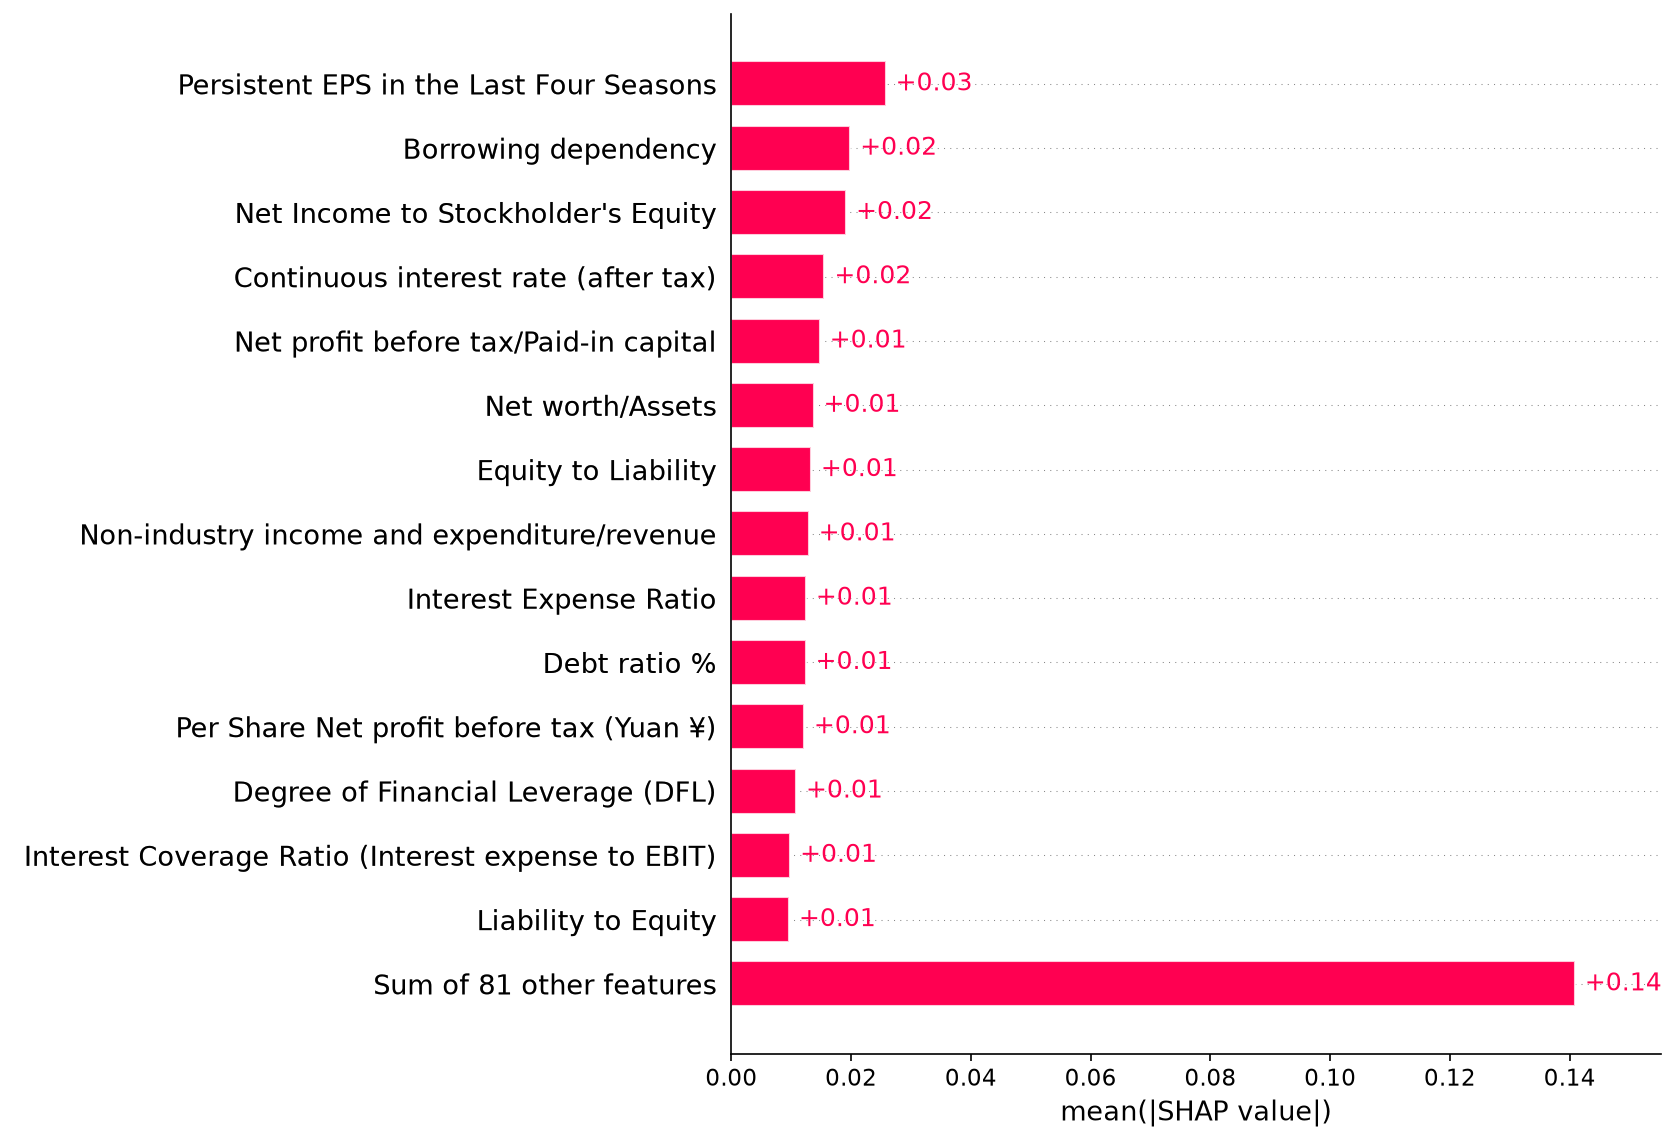
\includegraphics[width=0.82\textwidth]{shap_RandomForest_bar.png}
  \caption{Mean absolute SHAP values for the random forest.}
  \label{fig:shap-rf}
  \floatfoot{Source: own.}
\end{figure}

Permutation importance is led instead by leverage and interest measures, with the
Interest Expense Ratio first at $0.020$ and the rest of its values small
(Figure~\ref{fig:perm-rf}). Persistent EPS drops out of the ranking entirely. Its
closest earnings relatives, such as \emph{Net profit before tax/Paid-in capital} and
\emph{Per Share Net profit before tax}, are correlated with it above $0.95$, so when
it alone is shuffled they still carry almost the same information and the score barely
moves. This is the logic described in Section~\ref{sec:fi-permutation}, where
permutation hides a feature that has close substitutes and here it seems to hide the very
feature that native importance and SHAP both rank first.

\begin{figure}[htbp]
  \centering
  
\includegraphics[width=0.82\textwidth]{permutation_RandomForest.png}
  \caption{Permutation importance for the random forest, drop in $F_2$ when a feature
    is shuffled.}
  \label{fig:perm-rf}
  \floatfoot{Source: own.}
\end{figure}

Gradient Boosting is the best-performing model of the three and it produces the
clearest single ranking. Under SHAP the top feature is \emph{Borrowing dependency} at
$0.356$, a direct measure of how far a firm depends on debt, which had already risen
to second place under the random forest and now leads, ahead of Persistent EPS at
$0.292$. Native Gini importance still ranks Persistent EPS first, so SHAP overturns
the impurity ordering here.


\chapter{Discussion}
\label{ch:discussion}

The real-data undersampling approach and the comparison of three importance
methods across three models are the central contributions of this thesis. The
main result of that comparison is that the methods diverge, but they seem to do
so in an anticipated pattern, each showing the strengths and weaknesses that
were laid out throughout this thesis. The logistic regression is the simplest case. 
Because the $\ell_1$ penalty
already thinned most of the redundancy during training, all three methods agree
on the Debt ratio. This clean picture, however, comes from the weakest of the
three models. Whether a linear model can represent the full complexity of the
data remains open. The two ensembles predict better, but they receive the 
redundancy intact, since all $95$ features were deliberately kept for the integrity of the data and for
comparability with \textcite{wangliu2021}. Here the methods drift apart in
recognizable ways. The Gini ranking of the random forest carries three closely
related earnings measures on places one, three and four, which fits its described
tendency to split credit between near-identical features. Permutation drops
Persistent EPS entirely in both ensembles although the other methods rank it
first or second, which fits its described tendency to hide features with close
substitutes. SHAP, in turn, keeps the redundant families visible in every model,
which fits its described tendency to share credit between them. The redundancy
raised at the beginning therefore did not harm prediction, but it shaped
interpretation, as the disagreements between the methods concentrate largely
where features have near-identical partners. This consistency between what the
methods are known to do and what they visibly did here is the main insight of
the comparison. On its own each of these lists looks like the answer. 
Only the comparison shows that it is one of several, shaped by the model 
and the method behind it.

Read economically, and strictly as association rather than cause, the results
still tell one consistent story. Every model places a leverage measure at or
near the top, the Debt ratio for the logistic regression and Borrowing
dependency for the ensembles, so firms financed largely through borrowed capital
are the ones the models flag, which is also what one would expect economically.
At the same time the single most important feature is model-dependent, as the
random forest, nearly as strong as gradient boosting, ranks Persistent EPS first
under SHAP. Among the studies reviewed here, \textcite{sinap2025} is the only
other one applying SHAP to this dataset and reports Net Income to Total Assets,
in substance a return-on-assets measure, as the top feature of a stacking
classifier trained on SMOTE-balanced data and is followed by the Debt ratio. It is
notable that this list resembles the ranking of the linear model more than
those of the better-performing ensembles, where the Debt ratio sits far from
the top. Comparing these answers does not make one of them wrong. It shows that
a ranking depends on the whole pipeline that produces it, which supports
reading such lists with care.

The undersampling approach deserves the same two-sided reading. On the positive
side it achieves what it was chosen for. Every firm the models learned from
actually existed and the reported scores are measured on untouched test folds
with the natural $3.2\%$ bankruptcy rate, so they estimate the realistic case
honestly. This separates the results from the $98$--$99\%$ accuracies reported in
SMOTE-based studies, which train, and sometimes evaluate, on balanced data and
whose numbers therefore describe a different setting. The lower numbers here
reflect a more realistic task rather than weaker models. On the critical side,
undersampling discards information, as $5{,}939$ healthy firms enter each
training fold through only $660$ representatives. With roughly nine firms per
cluster, each representative is estimated from little data and would shift under
a new sample, a trade-off between representativeness and stability that the
repeated cross-validation softens but does not remove. 
The natural benchmark for this trade-off is \textcite{wangliu2021}, whose
framework this thesis leans on. Their best configuration reaches an $F_2$ of
$0.423$ where the best model here reaches $0.550$. This comparison is
encouraging but not exact, as the specifics of the pipelines still differ, for
example in the classifier itself. This is also why the thesis places its
contribution on the feature-importance layer rather than on performance alone.
What the comparison does show is that tree ensembles combined with
cluster-based undersampling, a combination \textcite{wangliu2021} left
unexplored, are worth the attention.
\clearpage
\chapter{Conclusion}
\label{ch:conclusion}

This thesis asked two questions, how well bankruptcy can be predicted when the
models learn from real firms only and which financial features the fitted
models then rely on. The first question is answered by the framework itself.
With ClusterCentroids undersampling, repeated stratified cross-validation and
the $F_2$-score as the selection metric, gradient boosting reaches an $F_2$ of
$0.550$ and the random forest $0.546$, both clearly ahead of the logistic
regression at $0.482$ and above the comparable result reported by
\textcite{wangliu2021}.

The answer to the second question is that there is no single ranking. 
Although the three importance methods diverge, they seem to do so along 
their known weaknesses, impurity importance splits credit between redundant 
features, permutation hides features with close substitutes and SHAP shares 
the credit while at the same time keeping it visible. Among these differences 
one signal remains stable, as each model puts a measure of debt dependence 
either at the top or very close to it. The contribution of the thesis therefore 
lies in the comparison. If each ranking were considered only on its own it would 
already seem to give the correct answer, it is only by placing them side by side 
that one can see how much of the ranking is influenced by the model and the method 
behind it.

Both of these contributions indicate the same direction for future research. Since 
the framework is not tied to this dataset, the natural next step is to apply it to 
data from other countries and markets in order to find out whether the undersampling 
approach holds and whether similar ratios appear under the importance methods. 
Datasets whose collection is documented more transparently would additionally allow 
first steps toward causal statements, which this thesis avoided carefully. 
Such data is rare, as collecting firm records of this scope is complex and costly, 
which is exactly why the well-studied benchmark Taiwanese dataset was chosen here. 
Until then, the value of this thesis lies in a pipeline whose results can be trusted 
for what they are, predictions and associations measured on real firms.



\newpage
\printbibliography
\newpage
\appendix
\chapter{Appendix}
\label{ch:appendix}

\section{Hyperparameter Search Spaces}
\label{sec:app-grids}

Table~\ref{tab:grids} lists the parameters searched for each model in the nested
grid search described in Section~\ref{sec:cv}. The three grids contain $12$, $36$
and $12$ combinations respectively, and since every combination is evaluated over
the full $30$ cross-validation fits, the search amounts to $1{,}800$ model fits in
total. The winning configurations are reported in Table~\ref{tab:selected} of
Section~\ref{sec:res-performance}.

\begin{table}[htbp]
  \centering
  \caption{Hyperparameter search spaces per model.}
  \label{tab:grids}
  \begin{tabular}{lll}
    \toprule
    \textbf{Model} & \textbf{Parameter} & \textbf{Values searched} \\
    \midrule
    \multirow{2}{*}{Logistic Regression}
      & \texttt{penalty}            & $\ell_1$, $\ell_2$ \\
      & \texttt{C}                  & $0.001$, $0.01$, $0.1$, $1.0$, $10.0$, $100.0$ \\
    \midrule
    \multirow{4}{*}{Random Forest}
      & \texttt{n\_estimators}      & $300$ (fixed) \\
      & \texttt{max\_depth}         & $3$, $5$, $10$ \\
      & \texttt{max\_features}      & \texttt{sqrt}, \texttt{log2}, $0.3$, $0.2$ \\
      & \texttt{min\_samples\_leaf} & $3$, $5$, $10$ \\
    \midrule
    \multirow{5}{*}{Gradient Boosting}
      & \texttt{n\_estimators}      & $200$ (fixed) \\
      & \texttt{learning\_rate}     & $0.05$, $0.1$ \\
      & \texttt{max\_depth}         & $1$, $2$, $3$ \\
      & \texttt{min\_samples\_leaf} & $1$, $5$ \\
      & \texttt{subsample}          & $0.8$ (fixed) \\
    \bottomrule
  \end{tabular}
  \floatfoot{Source: own.}
\end{table}

\section{Native Importance Rankings}
\label{sec:app-native}

Tables~\ref{tab:native-lr} to~\ref{tab:native-gb} list the top $15$ features by
native importance for each model, complementing the leading entries reported in
Section~\ref{sec:res-fi}. For the logistic regression the values are signed
coefficients, where a positive sign pushes the prediction toward bankruptcy. For
the two ensembles they are Gini impurity importances, which sum to one across all
features.

\begin{table}[htbp]
  \centering
  \caption{Native importance, logistic regression: top 15 signed coefficients.}
  \label{tab:native-lr}
  \small
  \begin{tabular}{rlr}
    \toprule
    & \textbf{Feature} & \textbf{Coefficient} \\
    \midrule
    1  & Debt ratio \%                          & $+14.493$ \\
    2  & ROA(B) before interest and depreciation after tax & $-9.558$ \\
    3  & ROA(A) before interest and \% after tax & $-5.193$ \\
    4  & Cash/Total Assets                      & $-4.738$ \\
    5  & Retained Earnings to Total Assets      & $+4.053$ \\
    6  & Total Asset Turnover                   & $-2.758$ \\
    7  & Total assets to GNP price              & $-2.678$ \\
    8  & Interest-bearing debt interest rate    & $-1.624$ \\
    9  & ROA(C) before interest and depreciation before interest & $-1.314$ \\
    10 & Tax rate (A)                           & $-1.219$ \\
    11 & After-tax net Interest Rate            & $+1.192$ \\
    12 & Liability-Assets Flag                  & $-0.997$ \\
    13 & Cash Turnover Rate                     & $-0.764$ \\
    14 & Fixed Assets Turnover Frequency        & $+0.569$ \\
    15 & Operating Profit Rate                  & $+0.565$ \\
    \bottomrule
  \end{tabular}
  \floatfoot{Source: own.}
\end{table}

\begin{table}[htbp]
  \centering
  \caption{Native importance, random forest: top 15 Gini impurity importances.}
  \label{tab:native-rf}
  \small
  \begin{tabular}{rlr}
    \toprule
    & \textbf{Feature} & \textbf{Importance} \\
    \midrule
    1  & Persistent EPS in the Last Four Seasons     & $0.092$ \\
    2  & Net Income to Stockholder's Equity          & $0.073$ \\
    3  & Net profit before tax/Paid-in capital       & $0.059$ \\
    4  & Per Share Net profit before tax (Yuan)      & $0.053$ \\
    5  & Continuous interest rate (after tax)        & $0.046$ \\
    6  & Borrowing dependency                        & $0.041$ \\
    7  & Net Income to Total Assets                  & $0.032$ \\
    8  & Total income/Total expense                  & $0.028$ \\
    9  & Non-industry income and expenditure/revenue & $0.027$ \\
    10 & Net worth/Assets                            & $0.025$ \\
    11 & Debt ratio \%                               & $0.025$ \\
    12 & Equity to Liability                         & $0.024$ \\
    13 & Interest Expense Ratio                      & $0.023$ \\
    14 & Degree of Financial Leverage (DFL)          & $0.022$ \\
    15 & Interest Coverage Ratio (Interest expense to EBIT) & $0.020$ \\
    \bottomrule
  \end{tabular}
  \floatfoot{Source: own.}
\end{table}

\begin{table}[htbp]
  \centering
  \caption{Native importance, gradient boosting: top 15 Gini impurity importances.}
  \label{tab:native-gb}
  \small
  \begin{tabular}{rlr}
    \toprule
    & \textbf{Feature} & \textbf{Importance} \\
    \midrule
    1  & Persistent EPS in the Last Four Seasons     & $0.247$ \\
    2  & Borrowing dependency                        & $0.105$ \\
    3  & Non-industry income and expenditure/revenue & $0.079$ \\
    4  & Net Income to Stockholder's Equity          & $0.052$ \\
    5  & Continuous interest rate (after tax)        & $0.048$ \\
    6  & ROA(C) before interest and depreciation before interest & $0.035$ \\
    7  & Degree of Financial Leverage (DFL)          & $0.034$ \\
    8  & Interest Coverage Ratio (Interest expense to EBIT) & $0.027$ \\
    9  & ROA(B) before interest and depreciation after tax & $0.026$ \\
    10 & Cash/Total Assets                           & $0.025$ \\
    11 & Inventory/Working Capital                   & $0.025$ \\
    12 & Equity to Liability                         & $0.023$ \\
    13 & Debt ratio \%                               & $0.021$ \\
    14 & Interest Expense Ratio                      & $0.021$ \\
    15 & Net worth/Assets                            & $0.015$ \\
    \bottomrule
  \end{tabular}
  \floatfoot{Source: own.}
\end{table}

\section{Complexity and Overfitting Curves}
\label{sec:app-complexity}

The following figures provide the overfitting check referenced in
Section~\ref{sec:cv}. For each model one complexity parameter is swept while all
remaining parameters are held at their grid-search optimum and training and
validation $F_2$ are traced across that sweep. The selected configurations of
Table~\ref{tab:selected} sit at or before the point where the validation curve turns
down or stagnates, which is what rules out overfitting at the chosen settings. As noted in
Section~\ref{subsec:gb}, the depth axis is not comparable across the random forest
and gradient boosting.

\begin{figure}[htbp]
  \centering
  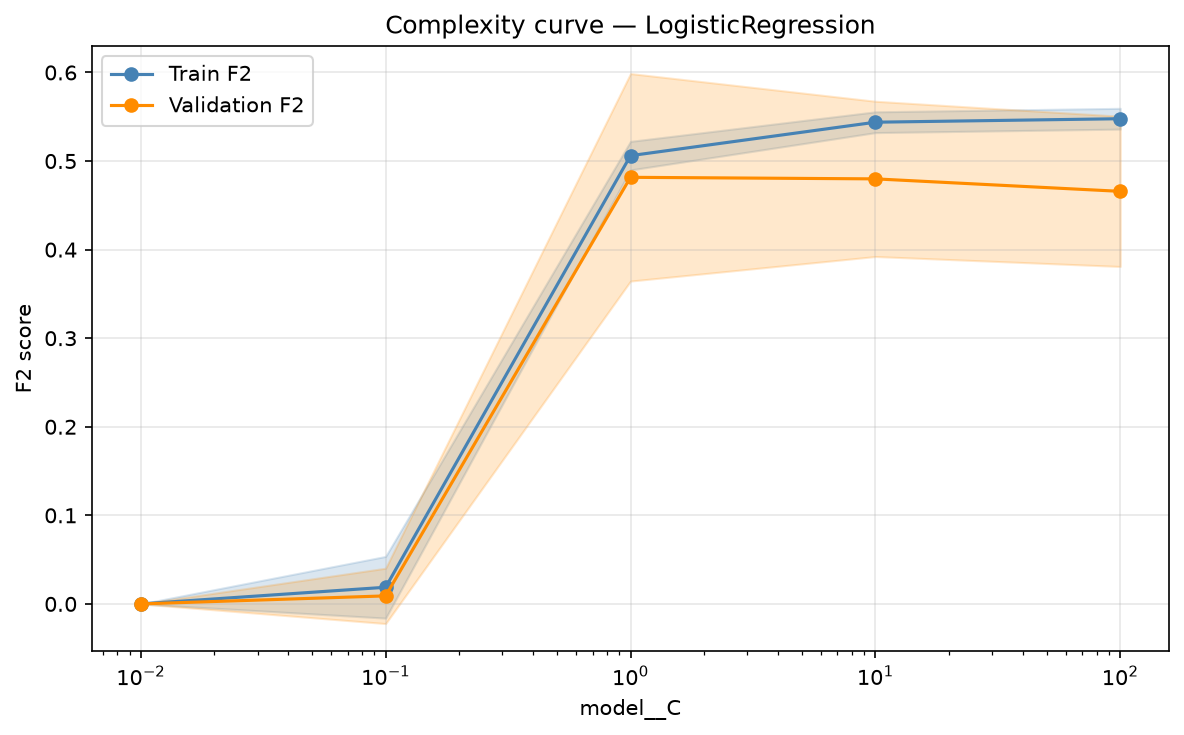
\includegraphics[width=0.75\textwidth]{complexity_curve_LogisticRegression.png}
  \caption{Logistic regression: training vs.\ validation $F_2$ across the inverse
    regularisation strength $C$, swept from $0.01$ to $100$ on a logarithmic axis.}
  \label{fig:cc-lr}
  \floatfoot{Source: own.}
\end{figure}

\begin{figure}[htbp]
  \centering
  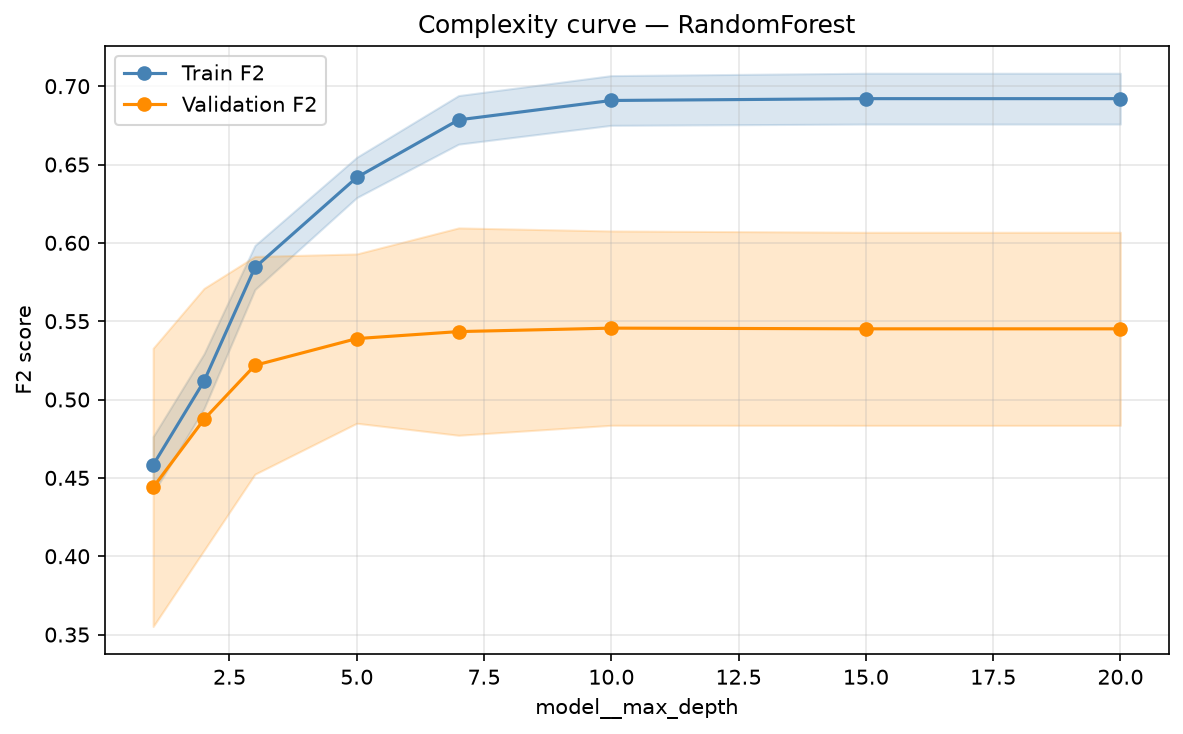
\includegraphics[width=0.75\textwidth]{complexity_curve_RandomForest.png}
  \caption{Random forest: training vs.\ validation $F_2$ across
    \texttt{max\_depth}, swept from $1$ to $20$.}
  \label{fig:cc-rf}
  \floatfoot{Source: own.}
\end{figure}

\begin{figure}[htbp]
  \centering
  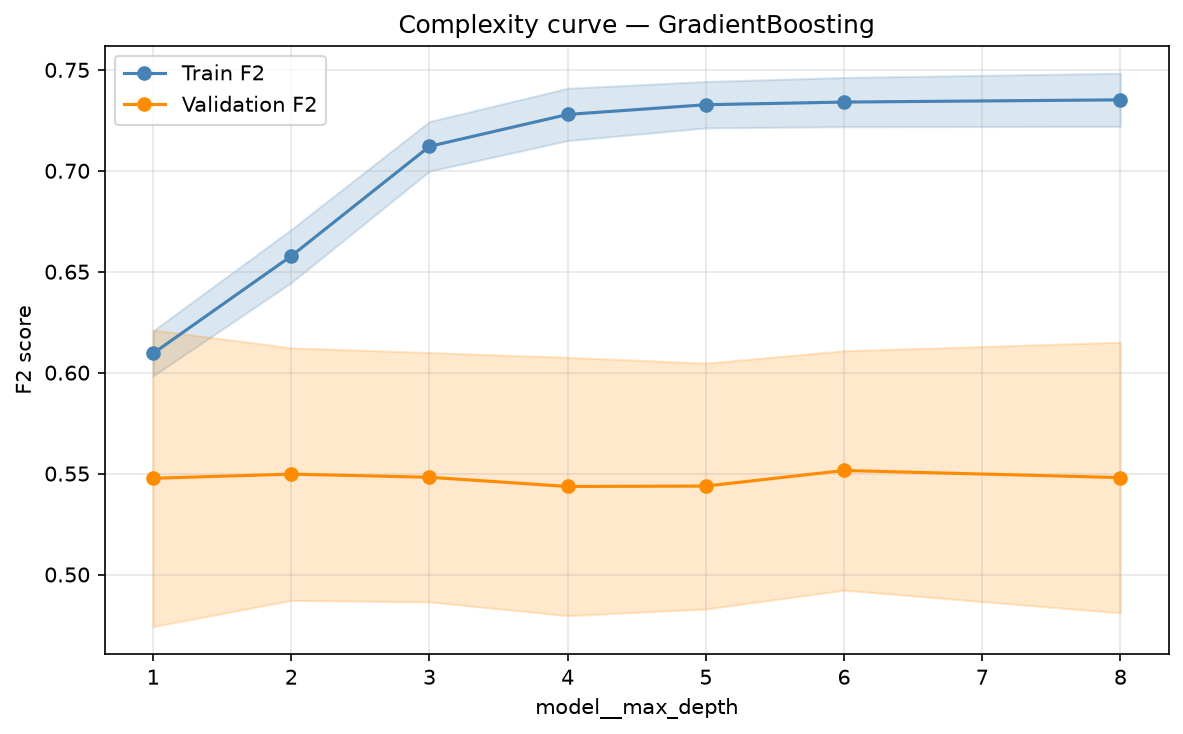
\includegraphics[width=0.75\textwidth]{complexity_curve_GradientBoosting.png}
  \caption{Gradient boosting: training vs.\ validation $F_2$ across
    \texttt{max\_depth}, swept from $1$ to $8$.}
  \label{fig:cc-gb}
  \floatfoot{Source: own.}
\end{figure}


\printthesisdisclaimer{Munich, 17.07.2026}{Niklas Demmrich}
\end{document}